%!TEX root=finmath2.tex
\chapter{Почему волатильность стохастическая?}
\chaptertoc

В этой лекции мы перечислим эмпирические факты, показывающие, что модель \bs\ не может адекватно описывать рыночные цены, и обсудим почему возникает необходимость в более продвинутых моделях, в которых волатильность задается случайным процессом.

\section{Напоминание: модель \bs}
В модели \bs\ цены безрискового и рискового активов задаются уравнениями
\[
d B_t = rB_t dt, \qquad
d S_t = \mu S_t dt + \sigma S_t d W_t.
\]
Для простоты будем считать, что рисковый актив не платит дивиденды, а безрисковая процентная ставка постоянна.
Решение уравнения для $S_t$ (геометрическое броуновское движение) представляется в виде
\[
S_t = S_0 e^{\sigma W_t + (\mu-\frac{\sigma^2}{2})t}.
\]

Для вычисления цен производных инструментов (платежных обязательств) нужно перейти к эквивалентной мартингальной мере $\Q$, относительно которой
\[
d S_t = r S_t dt + \sigma S_t d W_t^{\Q},
\]
где $W^{\Q}$ "--- броуновское движение относительно $\Q$.
Тогда цена европейского платежного обязательства в момент времени 0 с выплатой $X$, производимой  в момент $T$, вычисляется по формуле
\[
V = e^{-rT} \E^Q X.
\]
Для европейских опционов колл и пут математическое ожидание можно вычислить явно, что дает формулу \bs\ (см.~курс <<Введение в финансовую математику>>).
% \[
% \VC = S_0 \Phi(d_1) - K e^{-rT} \Phi(d_2), \qquad
% \VP = K e^{-rT} \Phi(-d_2) - S_0 \Phi(-d_1),
% \]
% где $\Phi(x)$ обозначает стандартную нормальную функцию распределения и
% \[
% d_1 = \frac{\ln(S_0/K) + (r+\sigma^2/2)T}{\sigma\sqrt T}, \qquad 
% d_2 = d_1 - \sigma\sqrt T.
% \]


\section{Почему модель \bs\ не согласуется с рыночными данными}
\subsection{Свойства вероятностных распределений рыночных цен}
\subsubsection{Отсутствие нормальности}

Для временного ряда рыночных цен с шагом $\Delta t$, \te\ $S_0, S_{\Delta t}, S_{2\Delta t},\dots$, построим последовательность
\[
L_t = \ln S_t - \ln S_{t-\Delta t}, \qquad t\in \{\Delta t, 2\Delta t,\dots\}.
\]
Если бы цены следовали модели \bs, то последовательность $L_t$ представляла бы реализацию последовательности независимых и одинаково распределенных нормальных случайных величин со средним $(\mu-\sigma^2/2)\Delta t$ и дисперсией $\sigma^2\Delta t$.

Из примера на рис.~\ref{intro:f:real-vol} видно, что это не так.
Левый график на этом рисунке изображает последовательность $L_t$ для индекса SnP~500 за 2015--2024 гг.\ с $\Delta t$ равным 1 дню, а правый график "--- симулированную последовательность нормальных величин с такими же средним и дисперсией. 
Характер графиков качественно отличается, что говорит о том, что распределение приращений значения индекса не является нормальным.
Аналогичная картина наблюдается и для других активов.

Ненормальность распределения подтверждается и гистограммой на рис.~\ref{intro:f:hist}.
Если бы данные были нормальными, то гистограмма была бы близка к графику плотности нормального распределения, но видно, что их формы отличаются.


\subsubsection{Ассимметрия и тяжелые хвосты}

Различие между эмпирическим распределением $L_t$ и нормальным распределением можно также увидеть из простых численных характеристик.
Например, вычислим выборочные коэффициенты асимметрии и эксцесса
\[
\gamma = \frac{\mu_3}{\sigma^3}, \qquad \kappa = \frac{\mu_4}{\sigma^4} - 3,
\] 
где $\mu_3,\mu_4$ "--- выборочные 3-й и 4-й центральные моменты, а $\sigma$ "--- выборочное стандартное отклонение.
Для выборки, полученной из нормального распределения, $\gamma$ и $\kappa$ будут близки к нулю (соответствующие теоретические коэффициенты для нормального распределения в точности равны 0), но в рассматриваемом примере с индексом SnP 500 получаются значения $-0.81$ и $15.7$.

Отрицательность коэффициента асимметрии говорит о том, что распределение скошено влево, а положительность коэффициента эксцесса "--- о том, что распределение имеет более <<тяжелые>> хвосты по сравнению с нормальным распределением.

\begin{figure}[t]
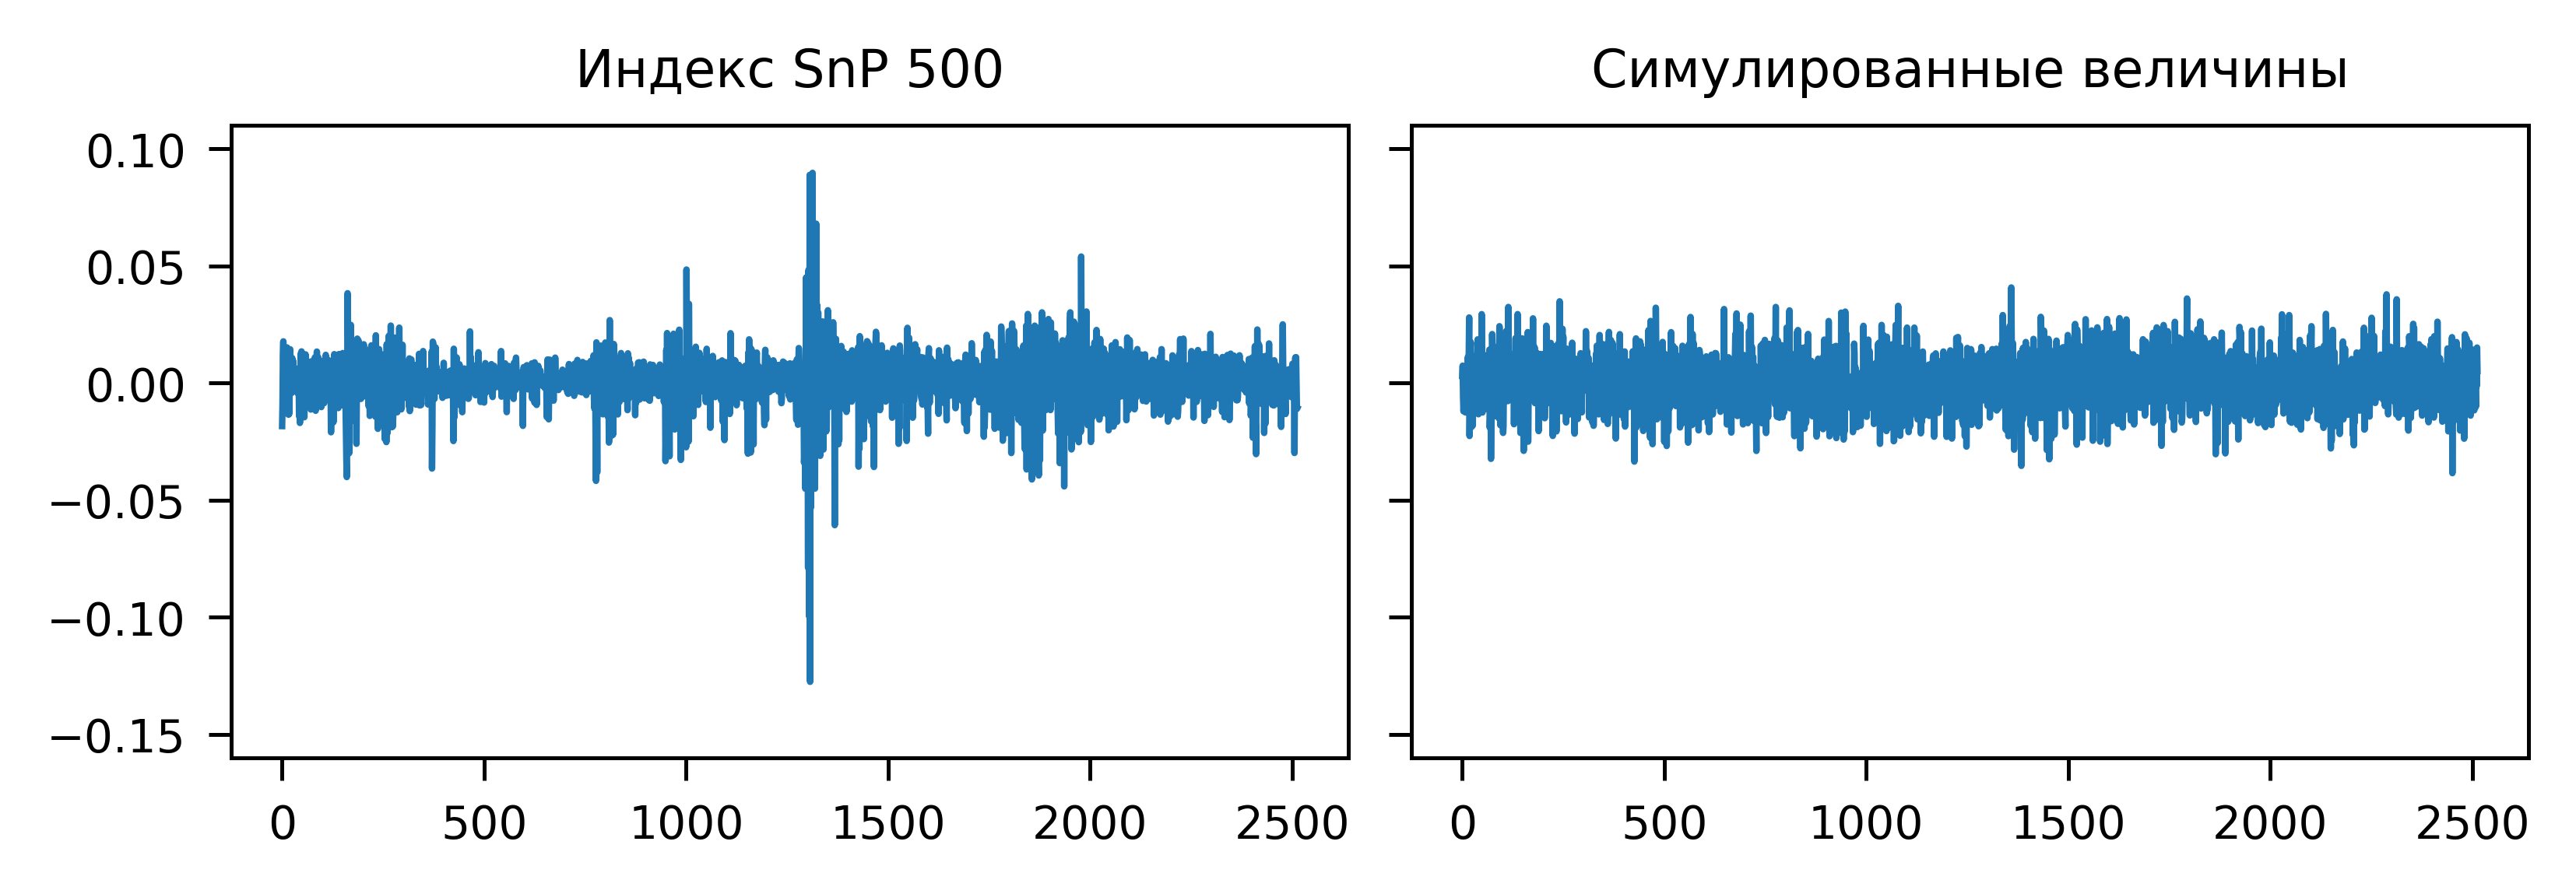
\includegraphics{pic/snp-returns.png}
\centering
\caption{Приращения логарифмов значений индекса SnP 500 и симулированные нормальные случайные величины с такими же средним и дисперсией.}
\label{intro:f:real-vol}
\end{figure}

\begin{figure}[t]
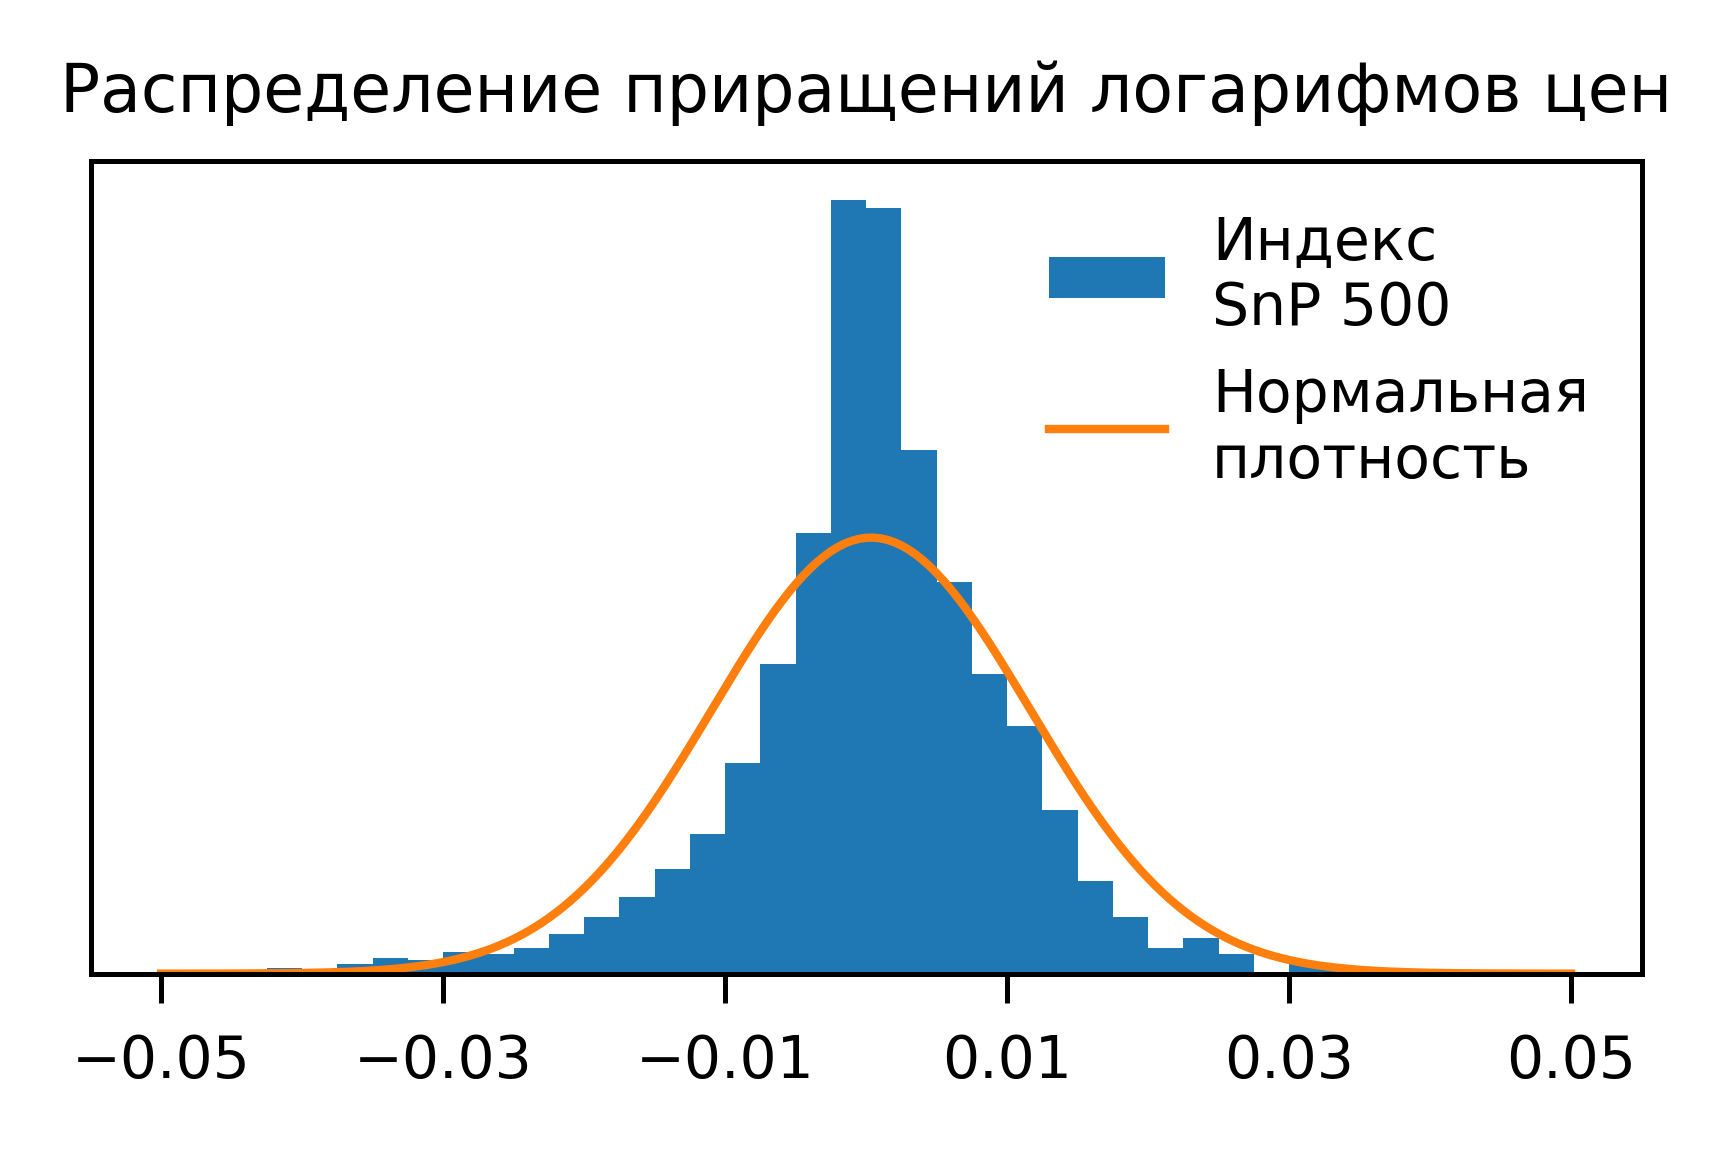
\includegraphics{pic/snp-hist.png}
\centering
\caption{Сравнение эмпирического распределения приращений логарифмов индекса SnP 500 с нормальным распределением.}
\label{intro:f:hist}
\end{figure}


\subsubsection{Автокорреляция}

Для геометрического броуновского движения величины $L_{t+s}$ и $L_t$ независимыми при $s\ge \Delta t$ в силу независимости приращений броуновского движения.
Из независимости следует некоррелированность, поэтому можно вычислить эмпирические коэффициенты корреляции (\te\ автокорреляционную функцию) и посмотреть, близки ли они к нулю.
Оказывается, что для рыночных данных корреляции $\rho(L_{t+s},L_t)$ близки к нулю, но корреляции квадратов приращений логарифмов $\rho(L_{t+s}^2,L_t^2)$ отличается от нуля (см.~рис.~\ref{intro:f:autocorr}).
Это говорит о том, что величины $L_{t+s}$ и $L_t$ зависимы, хотя и слабо коррелированны. 

\begin{figure}[t]
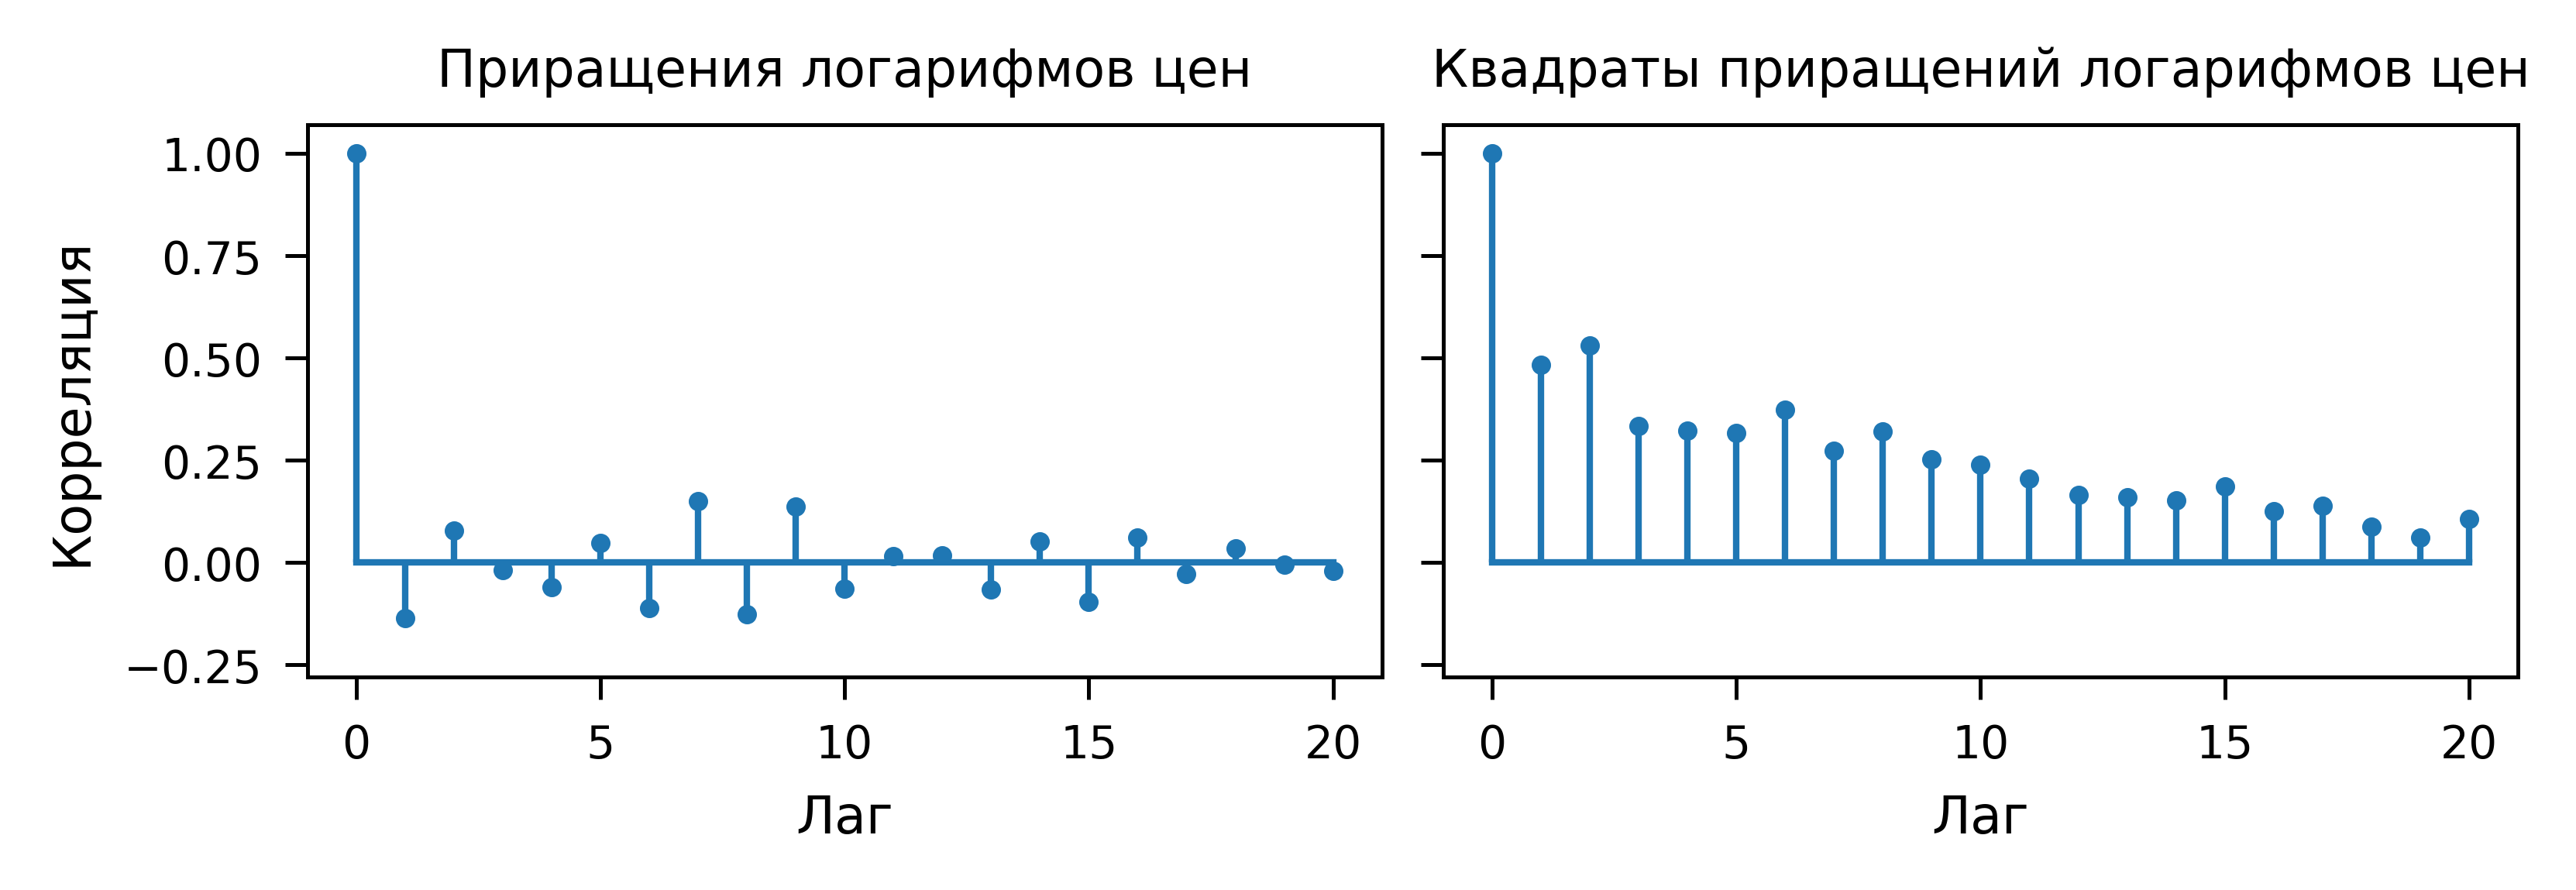
\includegraphics{pic/snp-autocorr.png}
\centering
\caption{Автокорреляционная функция для логарифмов приращений значения индекса SnP 500 и квадратов логарифмов приращений.}
\label{intro:f:autocorr}
\end{figure}


\subsubsection{Другие эмпирические факты}

Обзор статистических свойств рыночных цен приведен в статье \cite{Cont01}.
Эти свойства также называются \emph{стилизованными фактами}.
Кратко перечислим некоторые стилизованные факты, отсылая за подробностями к упомянутой статье.
\begin{itemize}
\item Имеется зависимость между изменениями цены и изменениями волатильности: часто при падении цены волатильность возрастает, а при росте цены остается без существенных изменений или плавно уменьшается. В модели \bs\ такого быть не может, так как величина $\sigma$ постоянна.

\item Кластеризация волатильности: за большими значениями волатильности преимущественно следуют большие значения, за малыми "--- малые.
Если представлять волатильность как степень <<беспокойства>> рынка, то это означает, что на рынке наблюдаются периоды спокойствия и беспокойства.
В модели \bs, напротив, рынок всегда <<одинаково спокоен>>.

\item Присутствие <<скачков>> (\te\ разрывов) в процессах цен, которые нельзя объяснить только тем, что данные собираются дискретным образом.%
\footnote{В этом курсе мы будем рассматривать модели, в которых процессы цен непрерывны.
Модели со скачками, основанные на \emph{процессах Леви}, были популярны в 2000-x гг.}
\end{itemize}


\subsection{Подразумеваемая волатильность}

На ликвидных рынках цены опционов можно считать известными (из рыночных данных), и тогда для каждого опциона можно найти значение $\sigma$ такое, что цена, вычисленная по формуле \bs, совпадает с рыночной ценой "--- это значение $\sigma$ называется \emph{подразумеваемой волатильностью}.
Мы будем обозначать его как $\hat\sigma(T,K)$, когда нужно подчеркнуть зависимость от страйка и времени исполнения.

Если бы рыночные данные следователи модели \bs, то построенная по ним функция $\hat\sigma(T,K)$ была бы постоянной и равнялась параметру волатильности в модели.
В реальности это не так.
Например, на рис.~\ref{intro:f:smiles} приведены \emph{улыбки волатильности}%
\footnote{Улыбкой волатильности называется функция $\hat\sigma(T,K)$, рассматриваемая как функция от страйка $K$ с фиксированным значением $T$.}
для опционов на индекс S\&P 500 с разными датами исполнения.
Видно, что функция $\hat\sigma(T,K)$ не постоянна как по $K$, так и по $T$.

Это приводит к трудности выбора параметра волатильности в модели \bs\ для оценки экзотических производных инструментов.
Например, следует ли для оценки барьерного опциона взять подразумеваемую волатильность, соответствующую страйку, равному барьеру, или страйку, равному текущей цене базового актива?
Хотелось бы иметь модель, которая позволяет оценивать деривативы, без изменения ее параметров под каждый инструмент.

\begin{figure}[t]
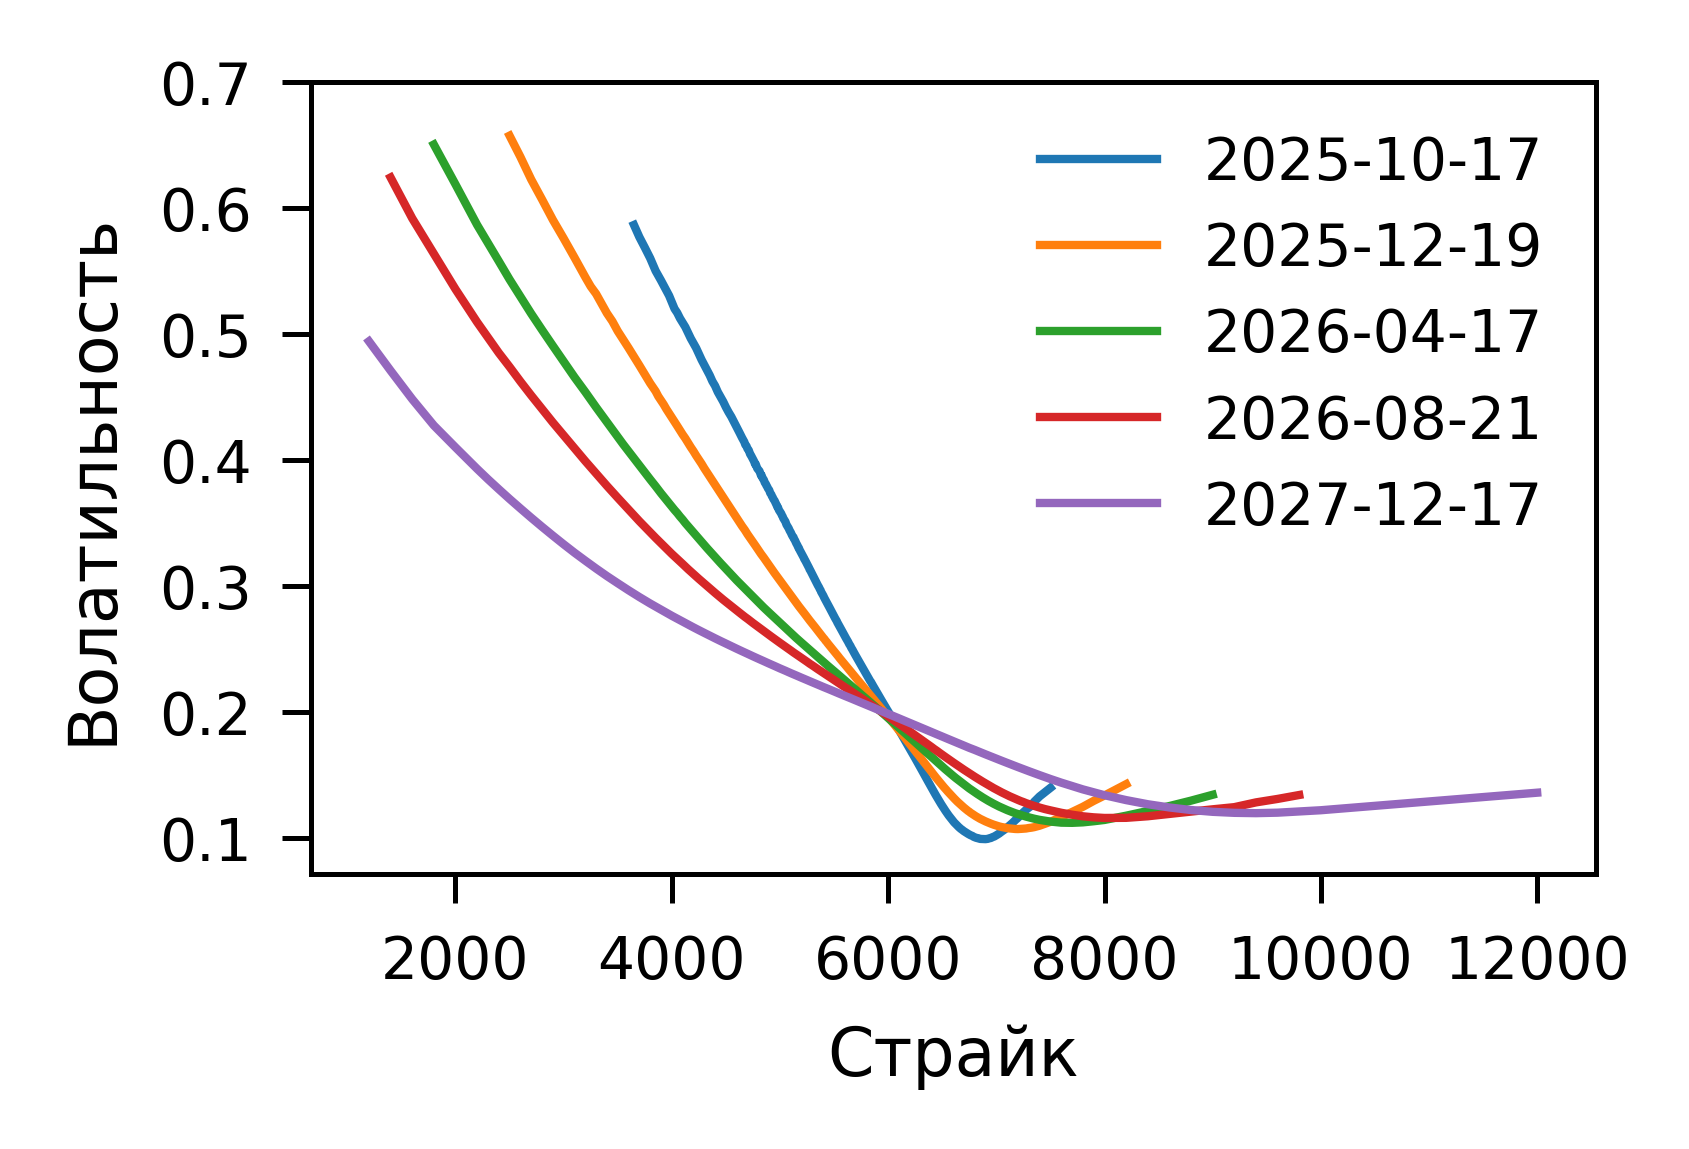
\includegraphics[height=5cm]{pic/snp-smiles.png}
\centering
\caption{Улыбки волатильности для индекса SnP 500 с разными датами исполнения, построенные по ценам опционов на дату  25.04.2024.}
\label{intro:f:smiles}
\end{figure}


\subsection{К каким ошибкам приводит модель \bs?}

Рассмотрим два типа ошибок, свойственных всем моделям и, в том числе, модели \bs.
Естественно, чем ошибка в модели меньше, тем модель лучше.
Соответственно, целью исследования более сложных моделей цен является, в том числе, нахождение моделей дающих меньшие ошибки.

\subsubsection{Статическая ошибка}
Под \emph{статической ошибкой} модели мы будем понимать несоответствие между рыночными ценами ликвидных (т.е.\ активно торгующихся и имеющих доступные рыночные цены) производных инструментов%
\footnote{Под ликвидными производными инструментами далее, в основном, имеются ввиду ванильные европейские опционы колл и пут.}
и ценами этих инструментов, получаемых в модели.

Статическая ошибка приводит к следующему нежелательному эффекту: модель дает цены инструментов, по которым их невозможно купить или продать.
Отметим, что статическая ошибка означает не то, что параметры модели неправильно откалиброваны к рыночным данным, а то, что модель в принципе не способна попасть в набор цен деривативов ни при каких комбинациях своих параметров.

В модели \bs\ статическая ошибка возникает из-за того, что в ней предполагается постоянство волатильности:
каким бы ни был параметр $\sigma$, модель не может воспроизвести рыночные улыбки волатильности, что означает невозможность воспроизвести рыночные цены ванильных опционов.


\subsubsection{Динамическая ошибка}

Под \emph{динамической ошибкой} мы будем понимать несоответствие между вероятностными распределениями процессов цен базовых активов, процессов цен ликвидных производных инструментов, а также других динамических характеристик%
\footnote{Например, такими характеристиками могут быть величины, вычисляемые из поверхности волатильности: волатильность опционов ATM, наклон и кривизна поверхности, и др.}, которые получаются в модели и наблюдаются в реальных данных. 

Динамическая ошибка приводит к ошибке репликации: производные инструменты, которые в выбранной модели теоретически можно реплицировать с помощью самофинансируемых стратегий, не реплицируются в точности.

Поясним на примере.
Пусть требуется реплицировать платежное обязательство, производящее выплату $X$ в момент времени $T$.
Для простоты предположим, что процентная ставка равна нулю, а $X$ зависит только от $S_T$, \te\ $X=f(S_T)$.
Если использовать для репликации модель \bs, то количество рискового актива $H_t$ в реплицируемом портфеле $\pi_t$ должно быть равно дельте инструмента:
\[
H_t = V'_s(t,S_t),
\]
где $V_t(t,s) = \E^{\Q} (f(S_T) \mid S_t=s)$ "--- его цена в модели \bs.
Тогда стоимость портфеля $\pi_t$ в момент исполнения будет равна
\[
V_T^\pi = V(0,S_0) + \int_0^T H_t d S_t = V(0,S_0) + \int_0^T V'_s(t,S_t) d S_t.
\]
С другой стороны, по формуле Ито имеем
\[
V(T,S_T) = V(0,S_0) + \int_0^T V'_t(t,S_t) dt + \int_0^T V'_s(t,S_t) d S_t + \frac12 \int_0^t V''_{ss}(t,S_t) (dS_t)^2.
\]
Так как $X=V(T,S_T)$, то для \emph{ошибки репликации} $\epsilon := V_T^\pi - X$ получаем выражение
\[
\epsilon = \int_0^T V'_t(t,S_t) dt + \frac12 \int_0^t V''_{ss}(t,S_t) (dS_t)^2.
\]

Далее воспользуемся тем, что $V'_t(t,s) = -\frac12 \sigma^2 V''_{ss}(t,s)$, как следует из уравнения \bs\ (при нулевой безрисковой ставке); здесь $\sigma$ "--- параметр волатильности в модели, используемой для репликации.
Если же допустить, что в реальности процесс цены $S_t$ имеет стохастическую волатильность, \te\ $dS_t = \sigma_t S_t d W_t$ со случайным процессом $\sigma_t$, то получим ненулевую ошибку:
\[
\epsilon = \frac12 \int_0^T (\sigma_t^2 - \sigma^2) V''_{ss}(t,S_t)S_t^2 dt.
\]

%%%%%%%%%%%%%%%%%%%%
% Старый фрагмент, непонятно написан
%%%%%%%%%%%%%%%%%%%%
% Рассмотрим функцию $V(t,S_t)$ такую, что $V(T,s) = g(s)$ (пусть пока $V$ произвольна, потом будет видно, как она связана с ценой платежного обязательства).
% Тогда портфель, состоящих из безрискового и рискового актива, стоимость которого в каждый момент времени равна $V(t,S_t)$, реплицирует $X$.
% Будем считать, что портфель не обязательно является самофинансируемым, и величина притока/оттока капитала описывается дифференциалом $C_t dt$.
% Тогда необходимо, чтобы было выполнено равенство $d V(t,S_t) = h_tdS_t + C_t dt$, где $h_t$ "--- количество единиц рискового актива в портфеле. По формуле Ито это эквивалентно равенству
% \[
% C_t dt = V'_t(t,S_t) dt + V'_s(t,S_t) dS_t + \frac12 V''_{ss}(t,S_t) (dS_t)^2 - h_t d S_t.
% \]
% Если выбрать $h_t=V'_s(t,S_t)$, то слагаемые с $dS_t$ сократятся, что уберет зависимость от изменения цены базового актива с точностью до первого порядка (<<дельта-хеджирование>>).
% Подставляя $(dS_t)^2 = \sigma^2 S_t^2 dt$, получаем
% \[
% C_t dt = \left(V'_t(t,S_t) + \frac{\sigma^2}2 V''_{ss}(t,S_t)S_t^2\right) dt.
% \]
% В модели \bs\ величина $\sigma$ постоянна.
% Поэтому, если предполагать, что модель верна, то можно найти функцию $V$ из уравнения в частных производных 
% \begin{equation}
% \label{intro:v}  
% V'_t + \frac{\sigma^2}{2} V''_{ss} = 0
% \end{equation}
% с терминальным условием $V(T,s) = f(s)$, что даст нулевой приток капитала $C_t$, и, таким образом, получится самофинансируемый портфель, который реплицирует $X$.

% Если же допустить, что волатильность $\sigma$ не постоянна, то получим (по-прежнему считая, что $V$ удовлетворяет \eqref{intro:v})
% \[
% C_t = \frac{\sigma_t^2-\hat\sigma^2}{2} V''_{ss}(t,S_t) S_t^2, 
% \]
% где $\hat\sigma$ "--- значение волатильности, которое использовалось при решении уравнения \eqref{intro:v}.
% Таким образом, денежная величина ошибки хеджирования составит
% \[
% C_T = \int_0^T \frac{\sigma_t^2-\hat\sigma^2}{2} V''_{ss}(t,S_t) S_t^2 dt.
% \]
% Тот факт, что $C_T$ не равно нулю означает наличие ошибки репликации.
% Она здесь возникла из-за того, что в модели предполагается постоянство коэффициента $\sigma$, а в реальности $\sigma_t$ не постоянно.
%%%%%%%%%%%%%%%%%%%%

\section{Краткая история моделей стохастической волатильности}

Под моделями стохастической волатильности мы будем понимать модели, в которых процесс цены базового актива относительно эквивалентной мартингальной меры имеет вид
\[
dS_t = r_tS_t dt + \sigma_t S_t dW_t,
\]
где $r_t$ "--- безрисковая процентная ставка (в этом курсе она будет, как правило, считаться детерминированной функцией), a $\sigma_t$ "--- случайный процесс\footnote{В случае, когда $\sigma_t$ является функцией только от текущего значения цены $S_t$ и времени, волатильность часто называют \emph{локальной}, а не стохастчиеской; см.~далее.}.
Замена постоянного параметра $\sigma$ в модели \bs\ на случайный процесс приводит к большому разнообразию получаемых моделей. 

Далее перечислим некоторые известные модели стохастической волатильности, кратко упомянув их достоинства и недостатки.
При первом чтении этого раздела многое может показаться непонятным.
К нему стоит вернуться после окончания курса.

\subsubsection{Модель CEV}

Первой моделью стохастической волатильности была \emph{модель CEV}\footnote{Constant Elasticity of Variance "--- модель c постоянной эластичностью дисперсии.}, предложенная Дж.~Коксом (J.~Cox, 1975).
Уравнение цены в ней имеет вид
\[
d S_t = r_tS_t dt + \sigma S_t^\gamma d W_t,
\]
где $\gamma \ge 0$ и $\sigma>0$ "--- параметры модели. Таким образом, здесь $\sigma_t = \sigma S_t^{\gamma-1}$. 
При $\gamma=1$ получается модель \bs, а при $\gamma=0$ "--- модель Башелье.

Если $\gamma\in[0,1)$, то волатильность растет, когда цена падает, и падает, когда, цена растет.
В первом приближении такое поведение действительно наблюдается в ценах акций.
Кроме того, улыбки волатильности в модели CEV при $\gamma\in(0,1)$ получаются скошенными вправо, что тоже в некоторой степени соответствует наблюдаемым данным.
Если $\gamma>1$, то получается противоположное поведение, которое не характерно для рынков акций, но, может наблюдаться, например, на рынках товаров.

У модели CEV имеется два недостатка.
Во-первых, она недостаточно гибкая, чтобы правильно описывать наблюдаемые поверхности подразумеваемой волатильности (у нее всего два параметра).

Во-вторых, функциональная зависимость $\sigma_t=\sigma(S_t)$ означает, что волатильность зависит только от текущего уровня цены, но в реальности на изменение волатильности оказывают влияние и другие факторы.
Можно провести такой мысленный эксперимент.
Пусть сегодня акция стоит 100, а через год будет стоить 120.
Если за этот год цена акции будет расти <<равномерно>> то можно ожидать, что к концу года волатильность будет в пределах своих <<обычных>> значений.
Однако, если за первые 11 месяцев цена вырастет до 180, а за последний месяц упадет до 120, то волатильность будет высокой. 
В модели CEV, напротив, в обоих случаях волатильность должна быть одинаковой.


\subsubsection{Модель локальной волатильности}

Модель локальной волатильности, предложенная Б.~Дюпиром (B.~Dupire, 1994), решает проблему статической ошибки: она в точности калибруется к ценам наблюдаемых европейских опционов.
Модель имеет вид
\[
d S_t = r_tS_t dt + \sigma(t,S_t) d W_t,
\]
где $\sigma(t,s)$ "--- детерминированная функция, которая определяется из рыночных цен опционов по некоторой аналитической формуле.

Несмотря на отсутствие статической ошибки, в модели локальной волатильности присутствует динамическая ошибка по той же причине, что и в модели CEV "--- из-за жесткой связи волатильности и цены.


\subsubsection{Модель Хестона}
Одной из наиболее известных моделей стохастической волатильности является модель C.~Хестона (S.~Heston, 1993).
Она задается уравнениями
\begin{align*}
&d S_t = r_tS_tdt + \sqrt{V_t} d W_t^{(1)},\\
&d V_t = \kappa(\theta - V_t)dt + \sigma \sqrt{V_t} d W_t^{(2)},\\
&d W_t^{(1)} d W_t^{(2)} = \rho dt,
\end{align*}
где процесс $V_t$ называется стохастической дисперсией (а $\sigma_t = \sqrt{V_t}$ "--- стохастической волатильностью).
Величины $\kappa,\theta,\sigma,\rho, V_0$ "--- параметры модели.
Третье уравнение означает, что броуновские движения $W_t^{(1)}$ и $W_t^{(2)}$ являются коррелированными с коэффициентом корреляции $\rho$ (\te\ $\E W_t^{(1)}W_t^{(2)} = \rho t$).

Пять параметров придают модели Хестона достаточно гибкости в подгонке к рыночным ценам опционов, но она все равно имеет статическую ошибку "--- это неизбежно при конечном числе параметров.
С другой стороны, зависимость волатильности от дополнительного случайного фактора позволяет более правильно отражать ее динамику по сравнению с моделью локальной волатильности. 

Большим достоинством модели Хестона является наличие эффективного способа вычисления цен европейских опционов, что необходимо для калибровки параметров модели.
Это важное свойство любой модели "--- можно придумать много разных уравнений, задающих стохастическую волатильность, но если нет эффективного метода вычисления цен простых деривативов, то такую модель модель будет трудно использовать на практике.

%%%%%%%%%%%%%%%%%%%%
%%% Непонятный абзац
%%%%%%%%%%%%%%%%%%%%
% Из недостатков модели Хестона можно отметить то, что она является недостаточно гибкой для описания динамики поверхности подразумеваемой волатильности.
% А именно, если откалибровать параметры модели по наблюдаемой поверхности подразумеваемой волатильности в текущий момент времени, то эти параметры будут также определять вероятностное распределение того, как вся поверхность будет двигаться в последующие моменты времени: грубо говоря, получается, что начальное значение процесса жестко связано с его распределением.
% Хотелось бы иметь параметры, которые будут отдельно контролировать динамику волатильности.
% Это необходимо для оценки экзотических деривативов, которые зависят от будущих значений волатильности (например, опционов с форвардным стартом). 

В дополнение к модели Хестона упомянем некоторые другие модели, в которых волатильность задается диффузионным процессом; эти модели не будут рассматриваться с нашем курсе, но они довольно обширно изучались в литературе: модель Халла"--~Уайта (Hull"--~White), модель Стейна"--~Стейна (Stein"--~Stein), модель 3/2.


\subsubsection{Модель SABR}

Другой хорошо известной моделью стохастической волатильности является модель SABR\footnote{Stochastic Alpha, Beta, Rho "--- стохастическая альфа, бета, ро.}, предложенная П.~Хэганом  соавторами (P.~Hagan, D.~Kumar, A.~Lesniewski, D.~Woodward, 2002):
\begin{align*}
&d S_t = r_t S_t dt + \alpha_t F_t^\beta d W_t^{(1)},\\
&d\alpha_t = \nu\alpha_t d W_t^{(2)},\\
&d W_t^{(1)} d W_t^{(2)} = \rho dt,
\end{align*}
где $\alpha_0,\beta,\nu,\rho$ "--- параметры модели.

Достоинство модели SABR состоит в том, что для нее имеется приближенная аналитическая формула для подразумеваемой волатильности, которая  позволяет быстро калибровать параметры модели и вычислять цены ванильных опционов.

Вообще, модель SABR часто используется не как динамическая модель, а именно как формула для интерполяции улыбок волатильности с учетом их динамики при изменении цены базового актива.
Под интерполяцией понимается то, что в реальности значения подразумеваемой волатильности даны в дискретном наборе точек (для разных страйков времен исполнения).

Поясним на примере.
Пусть $V(t,s,\sigma)$ "--- функция, задающая цену опциона по формуле \bs.
Чтобы получить его рыночную цену, вместо $\sigma$ нужно подставить подразумеваемую волатильность $\hat\sigma(t,s)$ этого опциона%
\footnote{Здесь параметры опциона $T,K$ фиксированы, но считается, что подразумеваемая волатильность зависит от времени и цены базового актива.
Может присутствовать зависимость и от других факторов, но для простоты мы сейчас ей пренебрежем.}.
Тогда, например, дельта опциона будет вычисляться как
\[
\Delta = \prt {V}s + \prt {V}\sigma \prt{\hat\sigma} s = \Delta_{BS} + \mathcal{V}_{BS} \prt{\hat\sigma} s,
\]
где $\Delta_{BS}$ и $\mathcal{V}_{BS}$ "--- дельта и вега в модели \bs.
Таким образом, возникает поправка в виде последнего члена, связанная с тем, что улыбка волатильности обладает динамикой (движется при изменении цены $s$).
Имея аналитическую формулу для $\hat\sigma$, эту поправку легко вычислить. 


\subsubsection{Модель SVI}

Модель SVI\footnote{Stochastic Volatility Inspired "--- модель, <<вдохновленная>> стохастической волатильностью.} (J. Gatheral, 1999) "--- это метод интерполяции и экстраполяции улыбок волатильности.
Она представляет из себя специально подобранную аналитическую функцию, зависящую от 5 параметров, которая хорошо <<ложится>> на рыночные улыбки волатильности.%
\footnote{Модель SVI не описывает динамику движения цен, \te, в общем-то, не является моделью стохастической волатильности.}

Задача интерполяции и экстраполяции волатильности является непростой по той причине, что желательно интерполировать и экстраполировать так, чтобы цены ванильных опционов, вычисленные по получаемой подразумеваемой волатильности, не приводили к наличию арбитража. 
При использовании общих методов (таких, как например, сплайны), добиться этого труднее, чем при использовании SVI.


\subsubsection{Модель Бергоми}

Модель Бергоми (L.~Bergomi, 2004--2005) позволяет более аккуратно моделировать динамику форвардной дисперсии, что важно для оценки экзотических опционов, зависящих от значений подразумеваемой волатильности в будущем.

В общем случае модель Бергоми порождается $n$ броуновскими движениями ($n$-факторная модель), но сейчас для простоты рассмотрим только ее 1-факторную версию.
Она задается уравнениями
\begin{align*}
&d S_t = r_tS_t dt + \sqrt{\xi_t^t} S_t d W_t^{(1)},\\
&d \xi_t^T = \omega e^{-k(T-t)} \xi_t^T d W_t^{(2)}, \quad T>0,\ t\in [0,T],\\
&dW_t^{(1)}dW_t^{(2)} = \rho dt.
\end{align*}
где $\omega,\kappa,\rho$ "--- параметры модели, а $\xi^T = (\xi_t^T)_{t\in[0,T]}$ "--- семейство процессов \emph{$T$"=форвардной дисперсии}, индексированных параметром $T>0$, задающим дату экспирации.

Под $T$-форвардной дисперсией на дату $t$ понимается случайная величина $\xi_t^T = \E^{\Q}(\sigma_T^2 \mid \F_t)$, \te\ условное ожидание квадрата стохастической волатильности в будущем. Для каждого $T$ получается свой процесс $\xi^T_t$ с временем $t\le T$. 
Если зафиксировать текущее время $t$, то получится кривая форвардной дисперсии $\xi_t^T$, $T\ge t$. 
Мгновенная стохастическая волатильность равна $\sigma_t = \sqrt{\xi_t^t}$.

Начальная кривая форвардной дисперсии $\xi^0$ является параметром модели и может быть оценена по рыночным данным.
Несмотря на то, что в каждый момент времени $t$ имеется континуум значений форвардной дисперсии $\xi_t^T$, $T\ge t$, вся кривая управляется всего одним броуновским движением $W_t$ (в $n$-факторной модели будет $n$ броуновских движений), что делает модель доступной для аналитических и численных расчетов.


\subsubsection{Модели грубой волатильности}

В 2010-x гг.\ в научной литературе получили популярность модели, где стохастическая волатильность задается процессами, которые имеет более хаотичные (грубые) траектории, чем диффузионные процессы.
Примером такой модели является
\begin{align*}
&d S_t = r_tS_t dt + \sigma_t S_t d W_t,\\
&\sigma_t = \sigma e^{\nu W_t^H}
\end{align*}
где $W_t^H = (W_t^H)_{t\ge0}$ "--- \emph{дробное} (или, еще говорят, \emph{фрактальное}) броуновское движение с параметром $H\in(0,1)$.
По определению, дробным броуновским движением называется гауссовский случайный процесс с нулевым средним и ковариационной функцией $\cov(W_t^H,W_s^H) = \frac12 (t^{2H} + s^{2H} - |t-s|^{2H}) $.
При $H=1/2$ получается стандартное броуновское движение.
С помощью параметра $H$ можно контролировать грубость траекторий: чем $H$ ближе к нулю, тем траектории грубее%
\footnote{Более точно: на любом конечном отрезке траектории процесса $W^H$ с вероятностью 1 непрерывны по Гёльдеру с показателем $H'$ для любого $H' < H$.}.

К идее грубой волатильности приводят два наблюдения.
Во-первых, статистический анализ внутридневных изменений цен показывает, что распределение реализованной волатильности за день обладает свойствами, которые не могут получиться у диффузионных процессов, но ими обладает, например, фрактальное геометрическое броуновское движение с малым показателем $H$ (со значением примерно $H=0.15$).
Во-вторых, в рыночных поверхностях подразумеваемой волатильности наблюдается такой эффект, что коэффициент наклона улыбки волатильности ведет себя примерно как $T^p$ при времени до исполнения $T$ близком к нулю, где значение показателя $p$ близко к $-1/2$.
Опять же, этого нельзя достичь в моделях, где волатильность задается диффузионным процессов, но можно, если она более грубая.

В литературе изучались разные модификации стандартных моделей на случай грубой волатильности: грубая модель Хестона, грубая модель SABR, грубая модель Бергоми и \tp\ 
Большим недостатком моделей грубой волатильности является сложность работы с ними аналитически и численно.
Это вызвано тем, что дробное броуновское движение не является ни марковским процессом, ни семимартингалом (за исключением случая $H=1/2$), и поэтому стандартные средства из стохастического анализа к нему не применимы.
К настоящему время в финансовой индустрии модели грубой волатильности так и не начали активно использоваться.


\subsubsection{Модели локальной стохастической волатильности}

Локальная стохастическая волатильность "--- это <<надстройка>> над какой"=либо моделью стохастической волатильности, заключающаяся в добавлении в коэффициент волатильности\emph{ функции левериджа $\ell(t,s)$}:
\[
d S_t = r_tS_t dt + \sigma_tS_t\ell(t,S_t) dW_t,
\]
где $\sigma_t$ "--- стохастическая волатильность, заданная конкретным процессом, зависящим от парамеров (например, как в модели Хестона, Бергоми и \tp), а функция левериджа $\ell(t,s)$ подбирается таким образом, чтобы исключить статическую ошибку.
Стохастическая часть модели (процесс $\sigma_t$) дает <<правильные>> динамические характеристики, а локальная часть (функция $\ell$) "--- статические.

Из результатов для модели локальной волатильности выводится, что $\ell$ выражается через условное математическое ожидание $\E(\sigma_t\mid S_t)$, что приводит к уравнению
\begin{equation}
\label{intro:lsv}
dS_t = rS_t dt + \sigma_t S_t f(t,S_t,\E(\sigma_t\mid S_t)) d W_t,
\end{equation}
где функция $f$ выписывается явно через поверхность локальной волатильности.
Это уравнение представляет собой стохастическое дифференциальное уравнение Маккина"--~Власова, \te\ уравнение в котором коэффициенты зависят от вероятностного распределения его решения.

Модели локальной стохастической волатильности являются современным <<стандартом>> в финансовой индустрии, особенно в задачах оценки деривативов, зависящих от нескольких базовых активов. 
Определенную трудность при работе с ними представляет калибровка локальной части, \te\ численное нахождение функции $\ell(t,s)$.
Более того, в настоящее время до конца не понятно, при каких условиях уравнение \eqref{intro:lsv} корректно задает модель, \te\ когда у него существует единственное решение, а также при каких условиях используемые численные методы сходятся к теоретическому решению. 


\summary
\begin{itemize}
\item Модель \bs\ неправильно описывает вероятностные распределения цен: в реальности приращения их логарифмов имеют распределение, отличное от нормального, обладают тяжелыми хвостами и зависимы.
\item Модель \bs\ также неправильно описывает поверхности подразумеваемой волатильности: в ней они плоские, а в реальности это не так.
\item Моделям присущи статические и динамические ошибки.
Первая означает несоответствие между рыночными ценами ликвидных производных инструментов и ценами этих инструментов в модели; вторая "--- несоответствие между вероятностными распределениями процессов цен базовых и производных инструментов, которые получаются в модели и наблюдаются в реальных данных. 
\end{itemize}
